

\tikzset{every picture/.style={line width=0.75pt}} %set default line width to 0.75pt        
\trimbox{0cm 0cm 0cm 1.8cm}{ 

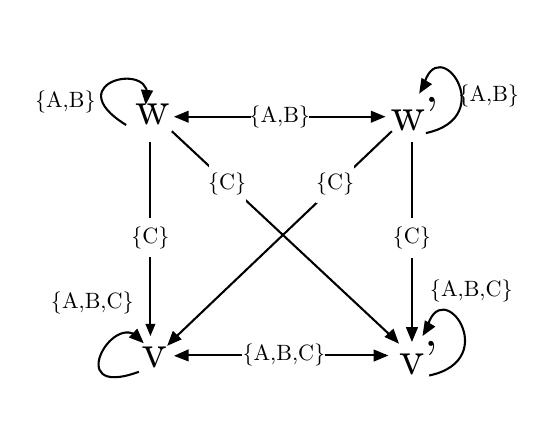
\begin{tikzpicture}[x=0.75pt,y=0.75pt,yscale=-1,xscale=1]
%uncomment if require: \path (0,237.1999969482422); %set diagram left start at 0, and has height of 237.1999969482422

%Straight Lines [id:da49380865843539024] 
\draw    (58,37.52) -- (58,129.88) ;


%Curve Lines [id:da5900505897070274] 
\draw    (55.82,18.4) .. controls (62.62,-2.4) and (11.9,8.32) .. (46.3,29.52) ;


%Shape: Triangle [id:dp7638941010979212] 
\draw  [fill={rgb, 255:red, 0; green, 0; blue, 0 }  ,fill opacity=1 ] (55.82,18.4) -- (54.11,12.94) -- (58.52,13.35) -- cycle ;
%Curve Lines [id:da33896708594278424] 
\draw    (53.81,133.72) .. controls (41.67,115.51) and (14.49,162.32) .. (52.43,148.41) ;


%Shape: Triangle [id:dp06181068467144124] 
\draw  [fill={rgb, 255:red, 0; green, 0; blue, 0 }  ,fill opacity=1 ] (53.81,133.72) -- (48.46,131.68) -- (51.51,128.48) -- cycle ;
%Straight Lines [id:da3518787636435954] 
\draw    (73.3,140.52) -- (171.3,140.52) ;


%Straight Lines [id:da9419961743422685] 
\draw    (167.3,25.52) -- (73.3,25.52) ;


%Straight Lines [id:da5282217469281014] 
\draw    (184,37.72) -- (184,130.08) ;


%Curve Lines [id:da1255493565606156] 
\draw    (191.12,127.8) .. controls (197.84,99.92) and (228.32,142.6) .. (192.32,150.2) ;


%Shape: Triangle [id:dp330887907957337] 
\draw  [fill={rgb, 255:red, 0; green, 0; blue, 0 }  ,fill opacity=1 ] (189.76,130.06) -- (190.59,124.4) -- (194.38,126.68) -- cycle ;
%Curve Lines [id:da19283464821040464] 
\draw    (189.52,11) .. controls (196.24,-16.88) and (226.72,25.8) .. (190.72,33.4) ;


%Shape: Triangle [id:dp48172892570830794] 
\draw  [fill={rgb, 255:red, 0; green, 0; blue, 0 }  ,fill opacity=1 ] (188.16,13.26) -- (188.99,7.6) -- (192.78,9.88) -- cycle ;
%Shape: Triangle [id:dp06884054633092584] 
\draw  [fill={rgb, 255:red, 0; green, 0; blue, 0 }  ,fill opacity=1 ] (184,132.72) -- (181.79,127.43) -- (186.21,127.44) -- cycle ;
%Shape: Triangle [id:dp349860096054311] 
\draw  [fill={rgb, 255:red, 0; green, 0; blue, 0 }  ,fill opacity=1 ] (171.3,140.58) -- (166.02,142.79) -- (166.02,138.37) -- cycle ;
%Shape: Triangle [id:dp5271852980265475] 
\draw  [fill={rgb, 255:red, 0; green, 0; blue, 0 }  ,fill opacity=1 ] (70.66,140.7) -- (75.94,138.31) -- (75.94,142.73) -- cycle ;
%Shape: Triangle [id:dp36308950352931935] 
\draw  [fill={rgb, 255:red, 0; green, 0; blue, 0 }  ,fill opacity=1 ] (58,129.88) -- (56.3,125.81) -- (59.7,125.81) -- cycle ;
%Shape: Triangle [id:dp1292227483684376] 
\draw  [fill={rgb, 255:red, 0; green, 0; blue, 0 }  ,fill opacity=1 ] (70.66,25.52) -- (75.94,23.31) -- (75.94,27.73) -- cycle ;
%Shape: Triangle [id:dp08607057312201727] 
\draw  [fill={rgb, 255:red, 0; green, 0; blue, 0 }  ,fill opacity=1 ] (169.94,25.52) -- (164.66,27.73) -- (164.66,23.31) -- cycle ;
%Straight Lines [id:da22782472852235425] 
\draw    (68.3,32.51) -- (176.84,133.88) ;


%Straight Lines [id:da40972295623496247] 
\draw    (174.3,32.51) -- (68.8,133.01) ;


%Shape: Triangle [id:dp9557525693039122] 
\draw  [fill={rgb, 255:red, 0; green, 0; blue, 0 }  ,fill opacity=1 ] (176.84,133.88) -- (171.64,131.49) -- (174.89,128.49) -- cycle ;
%Shape: Triangle [id:dp9360830131568407] 
\draw  [fill={rgb, 255:red, 0; green, 0; blue, 0 }  ,fill opacity=1 ] (66.99,134.94) -- (69,129.58) -- (72.22,132.61) -- cycle ;

% Text Node
\draw (59,24.32) node [scale=1.7280000000000002] [align=left] {\emphColorSlide{\poss{w}}};
% Text Node
\draw (59.8,141.22) node [scale=1.7280000000000002] [align=left] {\poss{v}};
% Text Node
\draw (17,18.32) node [scale=0.8] [align=left] {\{\agentSlide{A},\agentSlide{B}\}};
% Text Node
\draw (30,115.32) node [scale=0.8] [align=left] {\{\agentSlide{A},\agentSlide{B},\agentSlide{C}\}};
% Text Node
\draw (185.2,24.32) node [scale=1.7280000000000002] [align=left] {\poss{w'}};
% Text Node
\draw (187.11,141.72) node [scale=1.7280000000000002] [align=left] {\poss{v'}};
% Text Node
\draw (212.6,109.32) node [scale=0.8] [align=left] {\{\agentSlide{A},\agentSlide{B},\agentSlide{C}\}};
% Text Node
\draw (221,15.52) node [scale=0.8] [align=left] {\{\agentSlide{A},\agentSlide{B}\}};
% Text Node
\draw  [color={rgb, 255:red, 255; green, 255; blue, 255 }  ,draw opacity=1 ][fill={rgb, 255:red, 255; green, 255; blue, 255 }  ,fill opacity=1 ]  (106.8,16.52) -- (133.8,16.52) -- (133.8,34.52) -- (106.8,34.52) -- cycle  ;
\draw (120.3,25.52) node [scale=0.8,color={rgb, 255:red, 0; green, 0; blue, 0 }  ,opacity=1 ] [align=left] {\{\agentSlide{A},\agentSlide{B}\}};
% Text Node
\draw  [color={rgb, 255:red, 255; green, 255; blue, 255 }  ,draw opacity=1 ][fill={rgb, 255:red, 255; green, 255; blue, 255 }  ,fill opacity=1 ]  (49.5,74.7) -- (66.5,74.7) -- (66.5,92.7) -- (49.5,92.7) -- cycle  ;
\draw (58,83.7) node [scale=0.8,color={rgb, 255:red, 0; green, 0; blue, 0 }  ,opacity=1 ] [align=left] {\{\agentSlide{C}\}};
% Text Node
\draw  [color={rgb, 255:red, 255; green, 255; blue, 255 }  ,draw opacity=1 ][fill={rgb, 255:red, 255; green, 255; blue, 255 }  ,fill opacity=1 ]  (175.5,74.9) -- (192.5,74.9) -- (192.5,92.9) -- (175.5,92.9) -- cycle  ;
\draw (184,83.9) node [scale=0.8,color={rgb, 255:red, 0; green, 0; blue, 0 }  ,opacity=1 ] [align=left] {\{\agentSlide{C}\}};
% Text Node
\draw  [color={rgb, 255:red, 255; green, 255; blue, 255 }  ,draw opacity=1 ][fill={rgb, 255:red, 255; green, 255; blue, 255 }  ,fill opacity=1 ]  (86.5,48.7) -- (103.5,48.7) -- (103.5,66.7) -- (86.5,66.7) -- cycle  ;
\draw (95,57.7) node [scale=0.8,color={rgb, 255:red, 0; green, 0; blue, 0 }  ,opacity=1 ] [align=left] {\{\agentSlide{C}\}};
% Text Node
\draw  [color={rgb, 255:red, 255; green, 255; blue, 255 }  ,draw opacity=1 ][fill={rgb, 255:red, 255; green, 255; blue, 255 }  ,fill opacity=1 ]  (138.5,48.7) -- (155.5,48.7) -- (155.5,66.7) -- (138.5,66.7) -- cycle  ;
\draw (147,57.7) node [scale=0.8,color={rgb, 255:red, 0; green, 0; blue, 0 }  ,opacity=1 ] [align=left] {\{\agentSlide{C}\}};
% Text Node
\draw  [color={rgb, 255:red, 255; green, 255; blue, 255 }  ,draw opacity=1 ][fill={rgb, 255:red, 255; green, 255; blue, 255 }  ,fill opacity=1 ]  (102.8,131.52) -- (141.8,131.52) -- (141.8,149.52) -- (102.8,149.52) -- cycle  ;
\draw (122.3,140.52) node [scale=0.8,color={rgb, 255:red, 0; green, 0; blue, 0 }  ,opacity=1 ] [align=left] {\{\agentSlide{A},\agentSlide{B},\agentSlide{C}\}};


\end{tikzpicture}
}
